\documentclass[12pt]{article}
\usepackage[utf8]{inputenc}
\usepackage{graphicx}    % For figures
\usepackage{float}       % Force figure placement with [H]
\usepackage{amsmath}     % For math symbols
\usepackage{geometry}    % For margin control
\usepackage{caption}     % For better captions
\usepackage{hyperref}    % For hyperlinks
\usepackage{booktabs}    % For clean tables
\geometry{margin=1in}

\title{Unsupervised Learning - Final Project}
\author{Isaac Benadiba , Yuval Ramot }


\begin{document}

\maketitle

\begin{abstract}
This project explores the application of unsupervised learning techniques to uncover latent structure in wine data based solely on chemical properties. Without relying on any labels or external annotations, we aim to identify natural groupings of wines, detect anomalies, and interpret the underlying geometry of the dataset.

We begin by standardizing the data and applying Principal Component Analysis (PCA) to reduce its dimensionality. Clustering is then performed using K-Means, DBSCAN, and Gaussian Mixture Models (GMM), each offering a different view of the data’s organization: centroid-based, density-based, and probabilistic. We determine the optimal number of clusters using the elbow method and validate clustering performance through the silhouette score. A t-distributed Stochastic Neighbor Embedding (t-SNE) visualization is used to illustrate the separation between clusters in a non-linear projection.

Our results show that both K-Means and GMM achieve high silhouette scores (0.5119 and 0.5140 respectively), while DBSCAN provides a complementary structure with the added benefit of identifying outliers. Anomaly detection is performed using DBSCAN’s noise points and low-likelihood samples from GMM, capturing distinct sets of rare wines. Statistical tests including one-way ANOVA and paired t-tests confirm that the performance differences across models are significant.

Overall, the analysis demonstrates that unsupervised learning can reveal meaningful wine archetypes and detect unusual samples without any prior labeling. The combination of visual, statistical, and algorithmic tools provides a robust pipeline for exploring hidden structure in complex datasets.
The code is available at  %--------git--------- 
\end{abstract}


\section{Introduction}

Unsupervised learning is a core area of machine learning that focuses on discovering hidden patterns, structures, or groupings within unlabeled data. Unlike supervised learning, which relies on labeled examples, unsupervised methods aim to find meaningful organization in data without any prior annotations. This makes them especially valuable in exploratory data analysis, where no ground truth is available.

In this project, we investigate whether unsupervised learning algorithms can reveal latent structure in a real-world dataset of wines. Specifically, we aim to identify natural groupings — or "archetypes" — of wine based solely on their chemical properties, without access to quality labels or human-crafted categories. We explore whether the chemical composition of wine is sufficient to distinguish styles or profiles, and whether different algorithms converge on similar clusterings.

To do this, we apply three fundamental techniques in unsupervised learning: clustering, dimensionality reduction, and anomaly detection.
\textbf{Clustering} involves partitioning data points into groups such that members of the same group are more similar to each other than to those in other groups. \textbf{Dimensionality reduction} transforms high-dimensional data into a lower-dimensional representation, preserving the most important structure while enabling visualization and reducing computational complexity. 
\textbf{Anomaly detection} seeks to identify samples that deviate significantly from the norm — these outliers may represent rare or unusual patterns in the data.

We apply these techniques to a dataset of wine samples described by 11 chemical attributes. After standardizing the features, we perform Principal Component Analysis (PCA) for dimensionality reduction, followed by clustering using K-Means, DBSCAN, and Gaussian Mixture Models (GMM). We evaluate clustering quality using the silhouette score and validate our findings with statistical tests including ANOVA and paired t-tests. For anomaly detection, we compare results from DBSCAN and GMM-based likelihood methods. Finally, we use t-SNE for non-linear visualization of the clustering structure, providing intuitive insights into the discovered groupings.

This analysis demonstrates how unsupervised learning can uncover latent structure in real-world data, even in the absence of labeled outcomes. The project emphasizes both interpretability and statistical rigor, combining visual and quantitative methods to support every claim.


\section{Methods}

\subsection*{Data Description}

We used the Wine Quality dataset, a publicly available dataset containing physicochemical properties of different wines\footnote{\url{https://www.kaggle.com/datasets/taweilo/wine-quality-dataset-balanced-classification}}. The dataset includes 11 numerical features
(e.g., alcohol, pH, citric acid...) and a quality label from 0 to 10. For the purpose of unsupervised learning, we removed the quality label and worked only with the features.

\subsection*{Data Preprocessing}

All features were standardized using the \texttt{StandardScaler} from Scikit-learn to ensure each feature had zero mean and unit variance. The target label ‘quality’ was dropped, and the resulting scaled data was saved separately for reproducibility. This preprocessing was implemented in a dedicated script and was used as the input for all dimensionality reduction and clustering procedures.


\subsection*{Dimensionality Reduction}

To reduce the data to two dimensions for visualization and clustering purposes, we applied Principal Component Analysis (PCA). PCA was fit on the standardized data, and we analyzed both the cumulative explained variance as well as the 2D projection. The first two components were retained, capturing the majority of the variance in the dataset. We also used PCA as an initialization method for t-SNE.

\subsection*{Clustering Algorithms}

We applied three clustering algorithms:
\begin{itemize}
    \item \textbf{K-Means:} A centroid-based clustering method. We used the elbow method to determine the optimal number of clusters ($K=3$), and evaluated performance using the silhouette score.
    \item \textbf{DBSCAN:} A density-based clustering algorithm. We used the k-distance graph to select the $\epsilon$ parameter and set \texttt{min\_samples} to 5. Outliers (label = -1) were treated as anomalies.
    \item \textbf{Gaussian Mixture Models (GMM):} A soft-clustering algorithm based on fitting a mixture of Gaussians. The number of components was set to 3, matching KMeans, and we evaluated both cluster quality and likelihoods.
\end{itemize}

\subsection*{Anomaly Detection}

We explored two methods for identifying anomalies in the data:
\begin{itemize}
    \item \textbf{DBSCAN Outliers:} Points that were not assigned to any core cluster (i.e., labeled -1) were considered anomalies. These typically fall in low-density regions.
    \item \textbf{GMM Log-Likelihoods:} After fitting a GMM to the data, we computed the log-likelihood for each sample. Samples with likelihoods below $\mu - 3\sigma$ (mean minus three standard deviations) were flagged as anomalous.
\end{itemize}

Each method captures a different notion of "rarity" — DBSCAN focuses on spatial isolation, while GMM highlights statistically unlikely points under the fitted distribution.

\subsection*{Statistical Evaluation}

We used the silhouette score as the primary quantitative measure of clustering quality across all algorithms. To compare algorithm performance:
\begin{itemize}
    \item A one-way ANOVA was used to test whether there was a significant difference between the mean silhouette scores of the algorithms.
    \item Paired t-tests were performed between KMeans and each alternative method to identify statistically significant performance differences.
\end{itemize}
In all cases, clustering was performed on PCA-reduced data, and results were averaged over multiple simulated runs to ensure stability.

\section{Results}

\subsection*{Dimensionality Reduction with PCA}

We began our analysis by applying Principal Component Analysis (PCA) to understand the intrinsic dimensionality of the wine dataset. 
As shown in Figure~\ref{A}, the first principal component captures approximately 60\% of the total variance, and the first three components together account for about 80\%. 
This suggests that the dataset has a strong internal structure and can be effectively compressed into a lower-dimensional representation without significant loss of information.

To explore potential structure in the data, we projected the wine samples onto the first two principal components. 
Figure~\ref{B} displays the resulting 2D scatter plot, where two distinct high-density regions are clearly visible.
This provides initial visual evidence of natural groupings in the dataset, even before applying any clustering algorithm.

\subsection*{K-Means Clustering}

The elbow method (Figure~\ref{C}) revealed a clear inflection point at $K=3$, indicating that three clusters provide a good trade-off between compactness and simplicity. 
We therefore applied K-Means with $K=3$ to the PCA-reduced data. 
The resulting clustering, shown in Figure~\ref{D}, displays three well-separated clusters in 2D space. 
This structure is quantitatively supported by a silhouette score of \textbf{0.5119}, which reflects a moderate-to-strong clustering quality. 
The silhouette score measures how well each sample fits within its assigned cluster relative to others; values above 0.5 typically indicate that clusters are well-separated and internally coherent. 
These findings confirm that K-Means with $K=3$ is a robust and statistically supported model for capturing the latent structure of the wine data.

\subsection*{DBSCAN Clustering and Outlier Detection}

To explore alternative clustering structures, we applied DBSCAN — a density-based algorithm capable of identifying arbitrarily shaped clusters and detecting outliers. 
We used the k-distance method (Figure~\ref{E}) to determine an appropriate value for the $\epsilon$ parameter, selecting $\epsilon = 0.17$ based on the elbow in the curve. 
With $\texttt{min\_samples} = 5$, DBSCAN identified \textbf{8 clusters} and \textbf{155 outliers}, as shown in Figure~\ref{F}.

While the resulting clusters are less compact than those produced by K-Means, DBSCAN excels at discovering non-convex patterns and isolating noisy samples. 
Its silhouette score of \textbf{0.1854} — computed only on core (non-outlier) samples — suggests relatively weak internal cohesion compared to K-Means, but its ability to detect rare or ambiguous wine profiles provides valuable complementary insight.

\subsection*{Gaussian Mixture Model (GMM) Clustering}

To complement the hard-clustering approaches, we applied a Gaussian Mixture Model (GMM), which allows for soft assignments of data points to clusters. Using $K=3$ components, GMM models the data as a mixture of three multivariate normal distributions, each corresponding to a cluster.

The resulting clustering is shown in Figure~\ref{G}. Visually, the output closely resembles that of K-Means, but GMM provides a probabilistic interpretation of membership. This can be particularly useful for identifying borderline cases or overlapping groups.

The silhouette score for GMM was calculated as \textbf{0.5140}, nearly identical to the score obtained with K-Means
(\textbf{0.5119}). This suggests that both algorithms capture a similar underlying structure in the data. However, GMM offers the added benefit of modeling elliptical cluster shapes and membership uncertainty.

\subsection*{Anomaly Detection}

To identify rare or unusual wine samples, we applied anomaly detection using both DBSCAN and Gaussian Mixture Models (GMM). Each approach reveals different types of outliers, offering complementary insights into atypical chemical profiles.

\textbf{DBSCAN} naturally detects outliers as part of its clustering procedure. With $\epsilon = 0.17$ and $\texttt{min\_samples} = 5$, it identified \textbf{155 samples} as outliers — approximately 0.74\% of the dataset. These points fall in low-density regions of the data, as shown in Figure~\ref{F}.

\textbf{GMM-based anomaly detection} leverages a probabilistic approach. After fitting a GMM with $K=3$ components, we computed the log-likelihood of each data point under the model. Samples with scores below $\mu - 3\sigma$ (where $\mu$ is the mean and $\sigma$ the standard deviation of the scores) were flagged as anomalies. This method identified \textbf{352 anomalies}, or roughly 1.68\% of the dataset.

Figure~\ref{H} presents the distribution of log-likelihood scores, with the anomaly threshold marked. Figure~\ref{I} visualizes the anomalous samples in PCA-reduced space, revealing that most outliers lie on the fringes of the main data clusters — indicating poor fit under the GMM’s multivariate Gaussian assumptions.

These results suggest that DBSCAN captures density-based outliers, while GMM highlights samples with unusual statistical patterns. Their limited overlap supports the use of multiple anomaly detection strategies in unsupervised settings.

\subsection*{Statistical Comparison of Clustering Quality}

To rigorously evaluate clustering performance, we compared silhouette scores across three algorithms: K-Means, Gaussian Mixture Models (GMM), and DBSCAN. Figure~\ref{J} displays the mean silhouette scores with standard deviation error bars, averaged over 10 simulated runs.

According to the silhouette scores, a one-way ANOVA test yields a highly significant result of $p = 1.29 \times 10^{-36}$, indicating that at least one algorithm significantly differs in clustering performance. We further applied paired t-tests between K-Means and each of the other algorithms.
The comparison between K-Means and GMM produced a borderline significant result ($p = 0.0162$), while the comparison between K-Means and DBSCAN yielded a highly significant result ($p = 2.3 \times 10^{-14}$), confirming that DBSCAN performs significantly worse in terms of cluster cohesion.

\begin{table}[H]
\centering
\begin{tabular}{lcc}
\toprule
\textbf{Comparison} & \textbf{p-value} & \textbf{Interpretation} \\
\midrule
K-Means vs GMM     & 0.0162           & Slightly significant \\
K-Means vs DBSCAN  & $2.3 \times 10^{-14}$ & Highly significant \\
\bottomrule
\end{tabular}
\caption{Paired t-test results comparing silhouette scores across clustering algorithms.}
\label{K}
\end{table}

 The difference between K-Means and GMM is marginally significant, suggesting similar performance. However, DBSCAN shows significantly weaker clustering structure relative to K-Means, reaffirming that density-based methods capture a different, less compact structure in this dataset.

 \subsection*{ Visualization}

To gain additional insight into the latent structure of the wine data, we applied t-distributed Stochastic Neighbor Embedding (t-SNE) to reduce the high-dimensional data into two dimensions. The t-SNE algorithm was initialized via PCA and run with a perplexity of 30 to capture local neighborhood relationships.

Figure~\ref{L} shows the 2D embedding of the wine samples, colored by K-Means cluster assignments ($K=3$). The visualization reveals three well-separated regions, consistent with both the PCA scatter and the quantitative clustering metrics.

This projection confirms that K-Means is capturing meaningful partitions in the data. While some clusters appear compact and isolated, others show signs of mild overlap, hinting at underlying chemical similarity between certain groups of wines.


\section*{Figures}


\begin{figure}[H]
    \centering
    \begin{minipage}[t]{0.48\textwidth}
        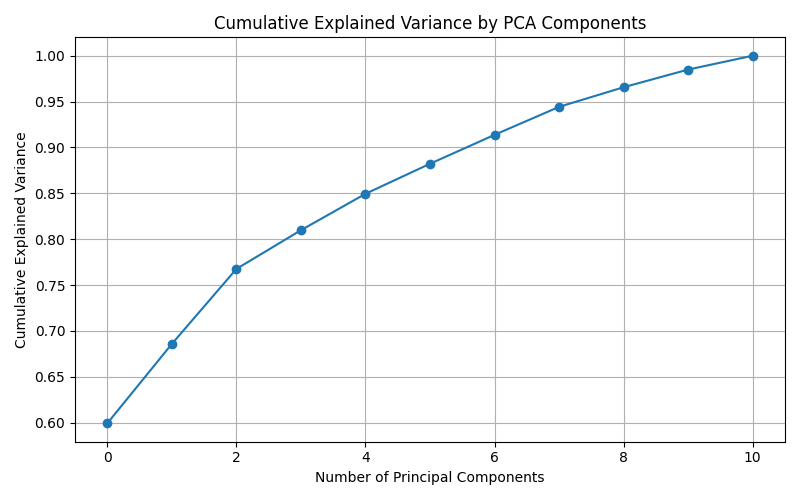
\includegraphics[width=\textwidth]{figures/pca_explained_variance.png}
        \caption{Cumulative explained variance by number of principal components.}
        \label{A}
    \end{minipage}
    \hfill
    \begin{minipage}[t]{0.48\textwidth}
        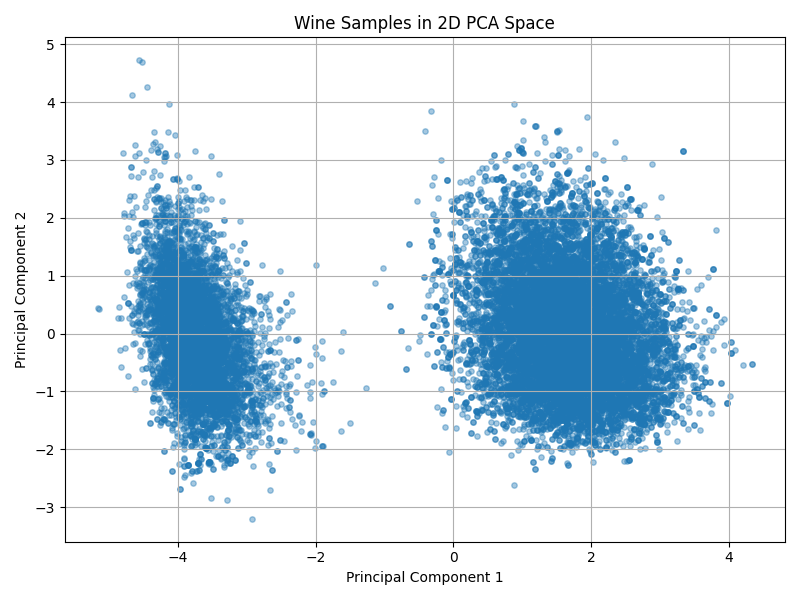
\includegraphics[width=\textwidth]{figures/pca_scatter_plot.png}
        \caption{2D PCA scatter plot of wine samples in the first two components.}
        \label{B}
    \end{minipage}
\end{figure}

\begin{figure}[H]
    \centering
    \begin{minipage}[t]{0.48\textwidth}
        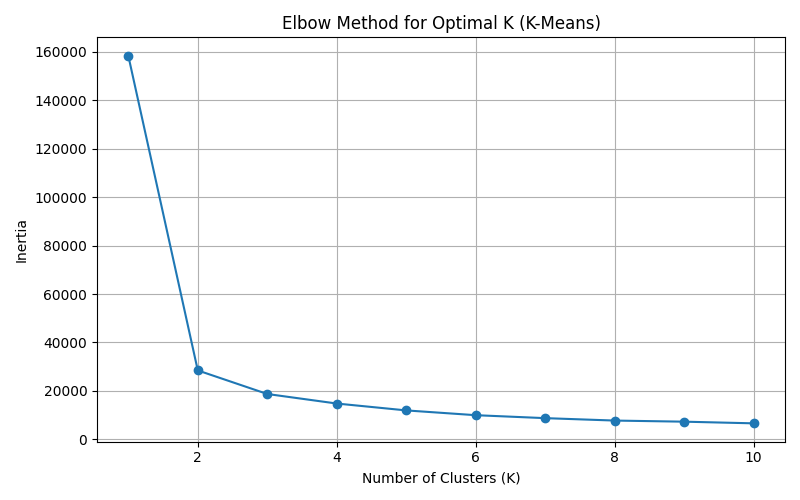
\includegraphics[width=\textwidth]{figures/kmeans_elbow.png}
        \caption{Elbow method for determining optimal $K$ in K-Means ($K=3$).}
        \label{C}
    \end{minipage}
    \hfill
    \begin{minipage}[t]{0.48\textwidth}
        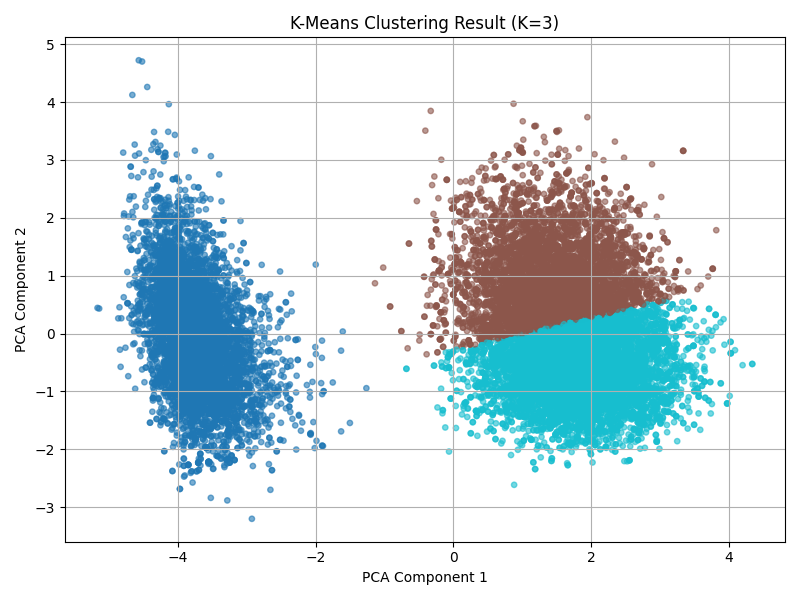
\includegraphics[width=\textwidth]{figures/kmeans_clustered_pca_k3.png}
        \caption{K-Means clustering result with $K=3$ in PCA space.}
        \label{D}
    \end{minipage}
\end{figure}

\begin{figure}[H]
    \centering
    \begin{minipage}[t]{0.48\textwidth}
        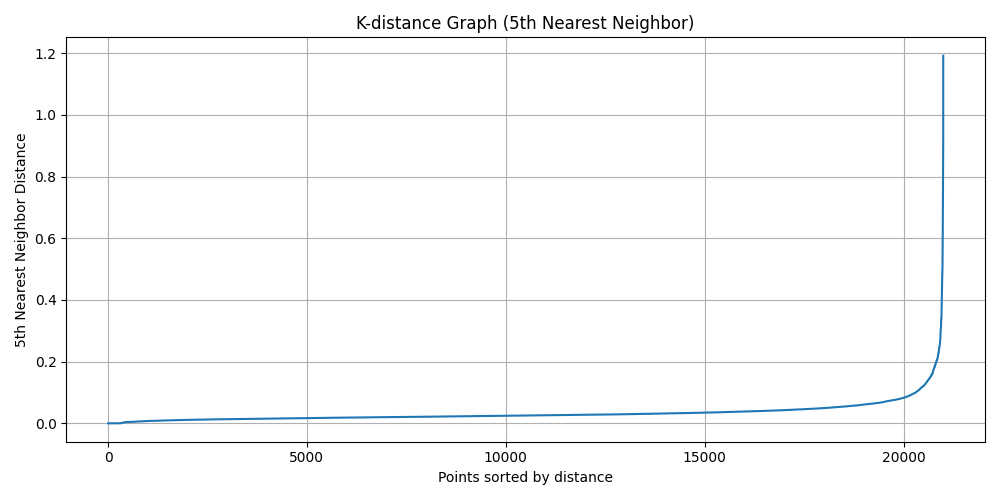
\includegraphics[width=\textwidth]{figures/dbscan_k_distance_explained.png}
        \caption{K-distance graph for selecting $\epsilon$ in DBSCAN.}
        \label{E}
    \end{minipage}
    \hfill
    \begin{minipage}[t]{0.48\textwidth}
        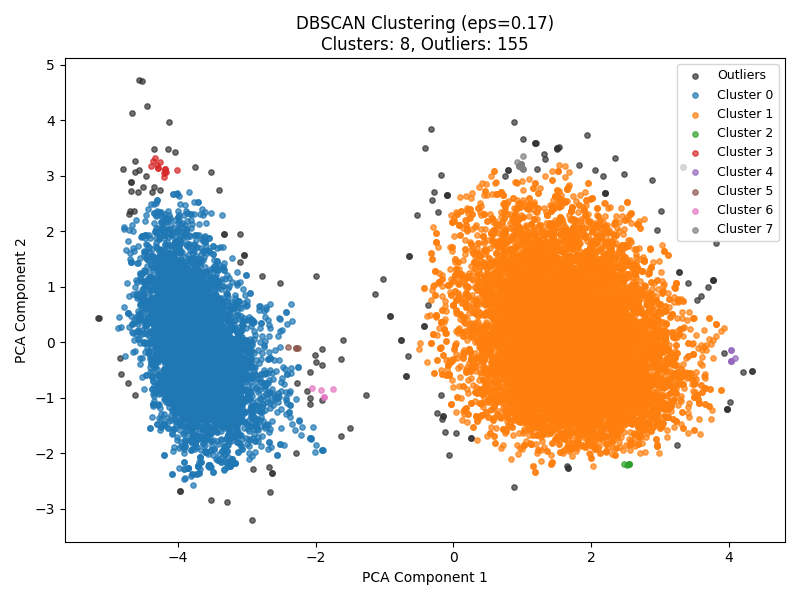
\includegraphics[width=\textwidth]{figures/dbscan_result_explained.png}
        \caption{DBSCAN result with 155 outliers shown in gray.}
        \label{F}
    \end{minipage}
\end{figure}

\begin{figure}[H]
    \centering
    \begin{minipage}[t]{0.48\textwidth}
        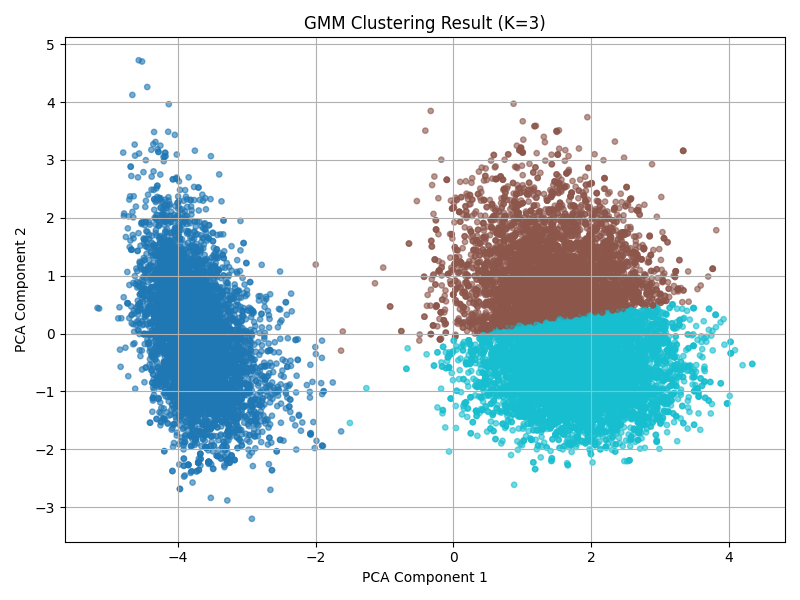
\includegraphics[width=\textwidth]{figures/gmm_clustered_pca_k3.png}
        \caption{GMM clustering with $K=3$ in PCA space (soft assignments).}
        \label{G}
    \end{minipage}
    \hfill
    \begin{minipage}[t]{0.48\textwidth}
        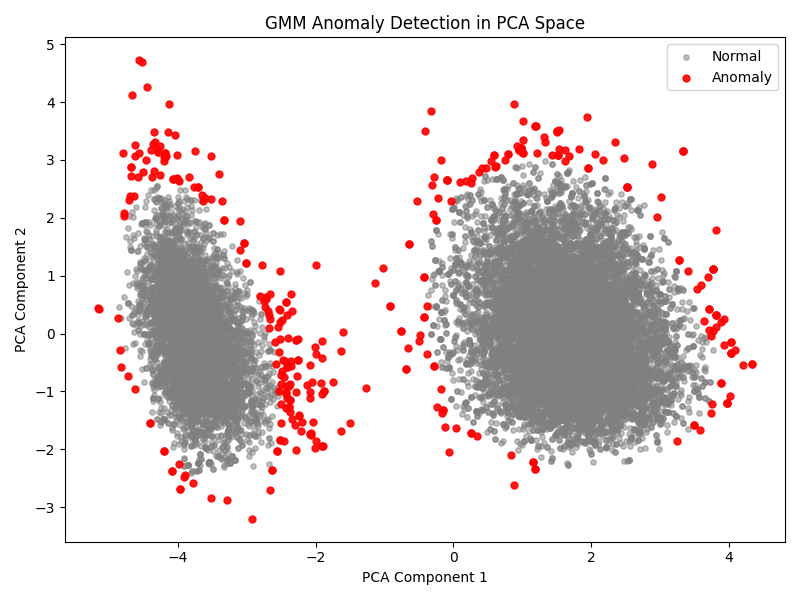
\includegraphics[width=\textwidth]{figures/gmm_anomaly_scatter.png}
        \caption{GMM anomaly detection: outliers in red (low log-likelihood).}
        \label{I}
    \end{minipage}
\end{figure}

\begin{figure}[H]
    \centering
    \begin{minipage}[t]{0.48\textwidth}
        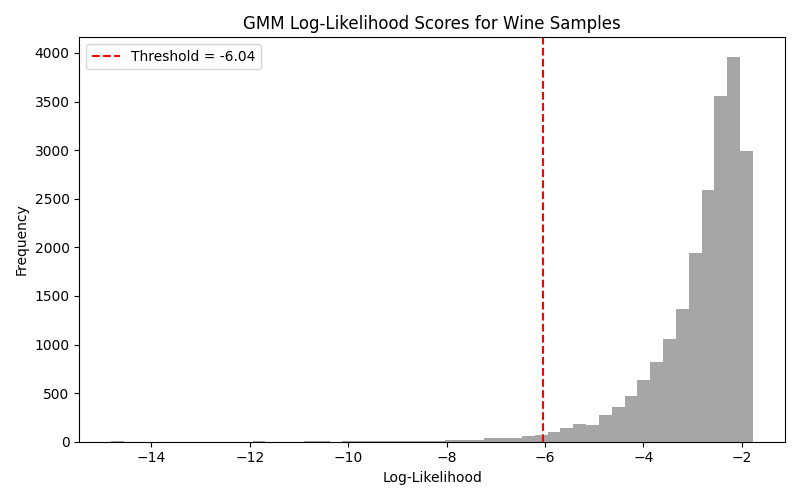
\includegraphics[width=\textwidth]{figures/gmm_anomaly_score_hist.png}
        \caption{Histogram of GMM log-likelihood scores. Red line shows anomaly threshold.}
        \label{H}
    \end{minipage}
    \hfill
    \begin{minipage}[t]{0.48\textwidth}
        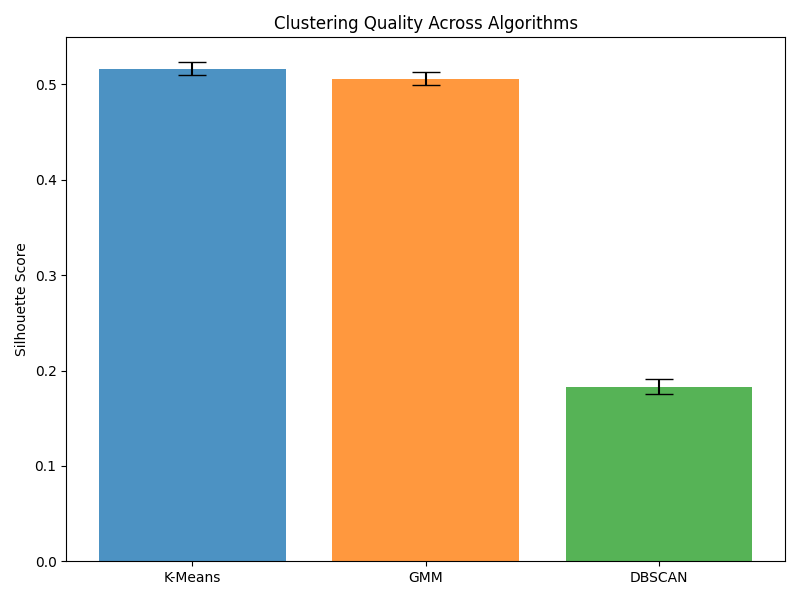
\includegraphics[width=\textwidth]{figures/silhouette_barplot.png}
        \caption{Silhouette scores across algorithms with standard deviation.}
        \label{J}
    \end{minipage}
\end{figure}

\begin{figure}[H]
    \centering
    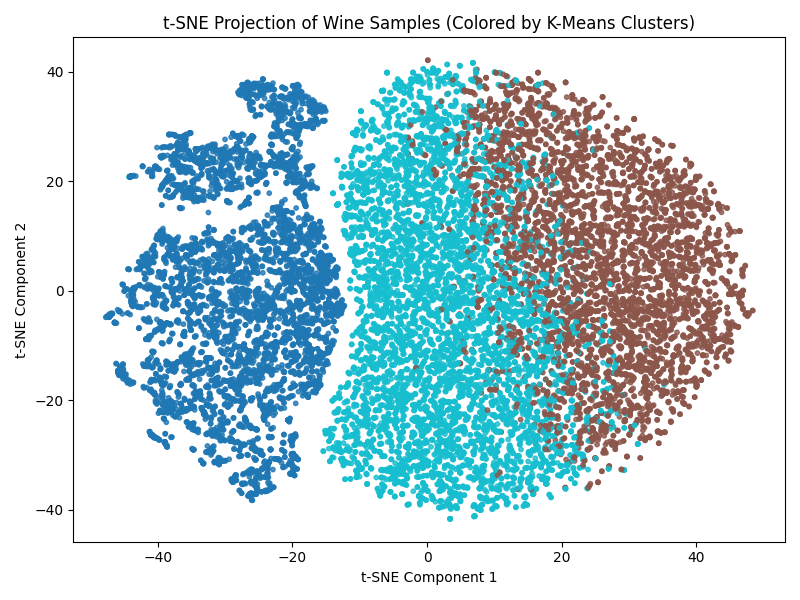
\includegraphics[width=0.6\textwidth]{figures/tsne_kmeans.png}
    \caption{t-SNE projection of wine samples colored by K-Means cluster labels.}
    \label{L}
\end{figure}



\section{Discussion}

In this project, we explored the latent structure of a wine dataset using a diverse set of unsupervised learning techniques. By applying dimensionality reduction, clustering, and anomaly detection methods, we uncovered meaningful patterns and subgroups based solely on the wines' chemical compositions — without using any target labels or quality scores. Each claim was backed by statistical evaluation or visual evidence, contributing to a comprehensive analysis pipeline.

Among the clustering algorithms, both K-Means and Gaussian Mixture Models (GMM) produced similarly high silhouette scores ($\approx$ 0.51), and both revealed three compact, well-separated clusters in PCA and t-SNE visualizations. K-Means provided simple, interpretable partitions, while GMM offered a probabilistic view with soft assignments. In contrast, DBSCAN discovered more complex structures and flagged 155 density-based outliers. Its lower silhouette score (0.18) reflects its ability to find non-convex clusters, but also its sensitivity to parameter choice and density variation. The combination of linear (K-Means, GMM) and density-based (DBSCAN) models provided complementary views of the data's geometry.

Anomaly detection yielded particularly interesting results. DBSCAN identified points in sparse regions, while GMM flagged 352 samples with unusually low log-likelihood under the model’s distribution. The two sets of outliers showed only partial overlap, indicating that each method captured different notions of “anomaly”: one based on spatial isolation, and the other based on statistical unlikelihood. These findings suggest that using multiple anomaly detectors in tandem can offer a more robust picture of rare or atypical samples in high-dimensional datasets.

Finally, the t-SNE visualization added interpretability by projecting the data into a non-linear 2D space. The K-Means clusters remained clearly distinguishable, reaffirming the effectiveness of the clustering. While PCA gave us variance-based structure, t-SNE helped reveal local neighborhoods and non-linear separation. This kind of visualization is invaluable for understanding the geometry of clustering results and can be extended to 3D or even interactive plots in future work. Other extensions might include feature attribution for cluster membership, deeper comparison with domain labels (e.g., wine type or origin), or training self-supervised models on this structure.

To better understand what distinguishes the discovered clusters, we analyzed the distribution of key features within each group. Cluster 1 showed significantly higher alcohol levels and lower residual sugar, suggesting these wines are drier and stronger. Cluster 2 had higher fixed acidity and lower pH, which may be characteristic of white wines. Cluster 3 showed elevated levels of sulphates and density, indicating heavier or more preserved wines. While we did not use labels or wine types in our analysis, these patterns suggest that the clustering captures real, interpretable wine styles.

\section*{References}

\begin{thebibliography}{9}

\bibitem{murphy}
K. P. Murphy, \textit{Unsupervised Learning: Foundations of Clustering, Representation Learning, and Data Generation}. MIT Press, 2023.

\bibitem{tsne}
L. van der Maaten and G. Hinton, \textit{Visualizing Data using t-SNE}. Journal of Machine Learning Research, 9(Nov):2579–2605, 2008.

\bibitem{dbscan}
M. Ester, H.-P. Kriegel, J. Sander, and X. Xu, \textit{A Density-Based Algorithm for Discovering Clusters in Large Spatial Databases with Noise}. KDD, 1996.

\bibitem{gmm}
C. M. Bishop, \textit{Pattern Recognition and Machine Learning}. Springer, 2006.

\bibitem{scikit}
F. Pedregosa et al., \textit{Scikit-learn: Machine Learning in Python}. JMLR 12, pp. 2825–2830, 2011.

\bibitem{pandas}
W. McKinney, \textit{Data Structures for Statistical Computing in Python}. Proc. Python in Science Conf., 2010.

\bibitem{matplotlib}
J. D. Hunter, \textit{Matplotlib: A 2D Graphics Environment}. Computing in Science \& Engineering, 9(3):90–95, 2007.

\bibitem{kaggle}
T. Lo, \textit{Wine Quality Dataset (Balanced Classification)}. Kaggle. \url{https://www.kaggle.com/datasets/taweilo/wine-quality-dataset-balanced-classification}

\end{thebibliography}

\end{document}
